\begin{dang}{Tìm tham số $m$ để hàm số đơn điệu trên các khoảng}
 \begin{listEX}
 \item Tìm tham số $m$ để hàm số bậc ba $y=ax^3+bx^2+cx+d$ đơn điệu trên tập xác định.
 \begin{itemize}
 \item \textbf{Bước 1:} Tìm tập xác định $\mathscr{D}=\mathbb{R}$. Tính đạo hàm $y'=3a x^2+2b x+c$, có \fbox{$\Delta'_{y'}=b^2-3ac$}
 \item \textbf{Bước 2:} Ghi điều kiện để hàm đơn điệu, chẳng hạn
 \begin{itemize}
 \item Để $f (x)$ đồng biến trên $\mathbb{R}\Rightarrow y'\geq 0,\forall x\in\mathbb{R}\Leftrightarrow\heva{&a_{y'}>0\\ &\Delta_{y'}\leq 0}\Rightarrow m$.
 \item Để $f (x)$ nghịch biến trên $\mathbb{R}\Rightarrow y'\leq 0,\forall x\in\mathbb{R}\Leftrightarrow\heva{&a_{y'}<0\\ &\Delta_{y'}\leq 0}\Rightarrow m $.
 \end{itemize}
 \end{itemize}
 \begin{note}
 Dấu của tam thức bậc hai $f(x)=a x^2+bx+c$.
 \begin{multicols}{2}
 \begin{itemize}
 \item $f(x)\geq 0,\forall x\in\mathbb{R}\Leftrightarrow\heva{&a>0\\ &\Delta\leq 0.}$
 \item $f(x)\leq 0,\forall x\in\mathbb{R}\Leftrightarrow\heva{&a<0\\ &\Delta\leq 0.}$
 \end{itemize}
 \end{multicols}
 \begin{itemize}
 \item Nếu hàm số $y=a x^3+b x^2+c x+d$ có $a$ chứa tham số thì chia ra hai trường hợp.
 \begin{itemize}
 \item Trường hợp $a = 0$ để xét tính đúng sai (nhận, loại m).
 \item Trường hợp $a\ne 0$ (sử dụng dấu tam thức bậc hai).
 \end{itemize}
 \end{itemize}
 \end{note}
 \item Tìm tham số $m$ để hàm số $y=\dfrac{ax+b}{cx+d}$ đơn điệu trên mỗi khoảng xác định của nó.
 \begin{itemize}
 \item \textbf{Bước 1:} Tìm tập xác định $\mathscr{D}=\mathbb{R}\backslash\left\{-\dfrac dc\right\}$. Tính đạo hàm $y'=\dfrac{ad-bc}{(c x+d)^2}$.
 \item \textbf{Bước 2:} Ghi điều kiện để hàm đơn điệu. Chẳng hạn
 \begin{itemize}
 \item Để $f (x)$ đồng biến trên mỗi khoảng xác định của nó $$\Rightarrow y'>0,\forall x\in\mathscr{D}\Leftrightarrow a d-b c>0\Rightarrow m. $$
 \item Để $f (x)$ nghịch biến trên mỗi khoảng xác định của nó $$\Rightarrow y'<0,\forall x\in\mathscr{D}\Leftrightarrow a d-b c<0\Rightarrow m.$$
 \end{itemize}
 \end{itemize}
 \item Tìm tham số $m$ để hàm số $y=\dfrac{a x+b}{c x+d}$ đồng biến trên $(\alpha ;\beta)$.
 \begin{itemize}
 \item \textbf{Bước 1: } Tìm điều kiện $x\neq-\dfrac dc$ và tính đạo hàm $y'=\dfrac{a d-c b}{(c x+d)^2}$.
 \item \textbf{Bước 2: } Hàm số đồng biến trên $(\alpha ;\beta)$ $$\Rightarrow\heva{&y'>0\\ &x\neq-\dfrac dc\\ &x\in(\alpha ;\beta)} \Leftrightarrow\heva{&a d-c b>0\\ &-\dfrac dc\notin(\alpha ;\beta)} \Leftrightarrow\heva{&a d-c b>0\\ & \hoac{&-\dfrac dc\leq\alpha\quad\Rightarrow m.\\ &-\dfrac dc\geq\beta}}$$
 \end{itemize}
 \item Xét hàm phân thức $y=\displaystyle\frac{ax^2+bx+c}{dx+e}$ có $y'=\dfrac{adx^2+2aex+be-dc}{(dx+e)^2}$, với $ad \ne 0$.
 \begin{itemize}
 \item [\ding{172}] Hàm số đồng biến trên từng khoảng xác định của nó khi và chỉ khi
 $$y'\ge 0,\, \forall x \ne -\dfrac{e}{d}\Leftrightarrow adx^2+2aex+be-dc\ge 0,\, \forall x \ne -\dfrac{e}{d}.$$
 \item [\ding{173}] Hàm số nghịch biến trên từng khoảng xác định của nó khi và chỉ khi
 $$y'\le 0,\, \forall x \ne -\dfrac{e}{d}\Leftrightarrow adx^2+2aex+be-dc\le 0,\, \forall x \ne -\dfrac{e}{d}.$$
 \end{itemize}
 \end{listEX}
\end{dang}
\begin{vd}%[2D1B1-3]
 Tìm $m$ để hàm số $y=f(x)=\dfrac{1}{3}x^3+mx^2+4x+3$ đồng biến trên $\mathbb{R}$.
 \loigiai{}
\end{vd}
\begin{vd}%[2D1B1-3]
 Tìm $m$ để hàm số $y=f(x)=-x^3-m x^2+(4 m+9) x+5$ nghịch biến trên khoảng $(-\infty ;+\infty)$.
 \loigiai{}
\end{vd}
\begin{vd}%[2D1B1-3]
 Tìm $m$ để hàm số $y=\dfrac{mx+4m}{x+m}$ nghịch biến trên từng khoảng xác định.
 \loigiai{}
\end{vd}
\begin{vd}%[2D1B1-3]
 Tìm $m$ để hàm số $y=\dfrac{m^2x-4}{x-1}$ đồng biến trên từng khoảng xác định.
 \loigiai{}
\end{vd}
\begin{vd}
 Tìm tất cả giá trị của tham số $m$ để hàm số
 $ y = \dfrac{2x^2+3x+m+1}{x+1} $ đồng biến trên các khoảng xác định.
 \loigiai{
 Tập xác định: $\mathbb{R}\setminus\{-1\}$.\\
 Ta có $y'=\dfrac{2x^2+4x+2-m}{(x+1)^2}$. Hàm số đồng biến trên các khoảng xác định khi
 $$2x^2+4x+2-m\ge 0, \forall x\in \mathbb{R} \Leftrightarrow m\le 0.$$
 }
\end{vd}
\begin{vd}
 Tìm tất cả giá trị của tham số $m$ để hàm số
 $y=\dfrac{x^2+(m+1)x-1}{2-x}$ nghịch biến trên mỗi khoảng xác định.
 \loigiai{
 Tập xác định $\mathscr{D}=\mathbb{R}\backslash{2}$.\\
 Đạo hàm: $y'=\dfrac{-x^2+4x+2m+1}{(2-x)^2}=\dfrac{g(x)}{(2-x)^2}$.\\
 Hàm số nghịch biến trên mỗi khoảng xác định của nó khi và chỉ khi $y'\le 0,\forall x\in \mathscr{D}$ (Dấu $'='$ chỉ xảy ra tại hữu hạn điểm thuộc $\mathscr{D}$).\\
 $\Leftrightarrow g(x)=-x^2+4x+2m+1\le 0,$ $\forall x\in \mathbb{R}$\\
 Điều kiện: ${\Delta}'\le 0$ (vì $a=-1<0$) $\Leftrightarrow 4-(-1)\cdot(2m+1)\le 0\Leftrightarrow 2m+5\le 0\Leftrightarrow m\le -\dfrac{5}{2}$.
 }
\end{vd}
\begin{vd}%[2D1B1-3]
 Tìm $m$ để hàm số $y=\dfrac{x-2}{x-m}$ đồng biến trên $(-\infty ;-1)$.
 \loigiai{}
\end{vd}
\begin{vd}%[2D1B1-3]
 Tìm $m$ để hàm số $y=\dfrac{2\cos x-1}{\cos x-m}$ đồng biến trên khoảng $\left(0;\dfrac{\pi}{2}\right)$.
 \loigiai{}
\end{vd}
\BTTN
\Opensolutionfile{ans}[ans/2D1-1-DANG-2]
\begin{ex}%[2D1K1-1]
 Có bao nhiêu giá trị nguyên của tham số $ m$ sao cho hàm số $ f(x)=\dfrac{1}{3}{x^3}+m{x^2}+4x+3$ đồng biến trên $\mathbb{R}$.
 \choice
 {\True $ 5$}
 {$ 4$}
 {$ 3$}
 {$ 2$}
 \loigiai{
 Ta có $f'(x)=x^2+2mx+4$.\\
 Hàm số đã cho đồng biến trên $\mathbb{R}$ khi và chỉ khi $f'(x)\ge 0,\forall x\in\mathbb{R}$ (Dấu ``$=$'' xảy ra tại hữu hạn điểm).\\
 Ta có $f'(x)\ge 0,\forall x\in\mathbb{R}\Leftrightarrow\Delta '\le 0$\\
 $\Leftrightarrow\Delta '=m^2-4\le 0$\\
 $\Leftrightarrow-2\le m\le 2$.\\
 Vì $ m\in\mathbb{Z}$ nên $ m\in\left\{-2;-1;0;1;2\right\}$, vậy có $ 5$ giá trị nguyên của $ m$ thỏa mãn.
 }
\end{ex}
\begin{ex}%[2D1K1-1]
 Cho hàm số $ y=-x^3-m{x^2}+\left(4m+9\right)x+5$, với $m$ là tham số. Hỏi có bao nhiêu giá trị nguyên của $m$ để hàm số nghịch biến trên khoảng $\left(-\infty ;+\infty\right)$
 \choice
 {$ 5$}
 {$ 4$}
 {$ 6$}
 {\True $ 7$}
 \loigiai{
 Tập xác định $\mathscr{D}=\mathbb{R}$\\
 $ y'=-3x^2-2mx+4m+9$.\\
 Hàm số nghịch biến trên $\left(-\infty ;+\infty\right)$ khi $y'\le 0,\forall x\in\left(-\infty ;+\infty\right)$ $\Leftrightarrow\left\{\begin{aligned}
 & a=-3<0\\
 &\Delta '=m^2+3\left(4m+9\right)\le 0\\
 \end{aligned}\right.$\\
 $\Leftrightarrow m\in\left[-9;-3\right]$ $\Rightarrow $ có $7$ giá trị nguyên của $m$ thỏa mãn.
 }
\end{ex}
\begin{ex}%[2D1K1-1]
 Cho hàm số $ y=-\dfrac{1}{3}{x^3}+m{x^2}+\left(3m+2\right)x+1$. Tìm tất cả giá trị của $ m$ để hàm số nghịch biến trên $\mathbb{R}$.
 \choice
 {$\left[\begin{aligned}
 & m\ge-1\\
 & m\le-2\\
 \end{aligned}\right.$}
 {\True $-2\le m\le-1$}
 {$-2<m<-1$}
 {$\left[\begin{aligned}
 & m>-1\\
 & m<-2\\
 \end{aligned}\right.$}
 \loigiai{
 Tập xác định $\mathscr{D}=\mathbb{R}$, $y'=-x^2+2mx+3m+2$ .\\
 Hàm số nghịch biến trên $\mathbb{R}$ khi và chỉ khi $y'\le 0$, $\forall x\in\mathbb{R}$\\
 $\Leftrightarrow\left\{\begin{aligned}
 & a=-1<0\\
 &{\Delta}'=m^2+3m+2\le 0\\
 \end{aligned}\right.$ $\Leftrightarrow-2\le m\le-1$.
 }
\end{ex}
\begin{ex}%[2D1K1-1]
 Tìm $ m$ để hàm số $ y=x^3-3m{x^2}+3\left(2m-1\right)+1$ đồng biến trên $\mathbb{R}$.
 \choice
 {Không có giá trị $ m$ thỏa mãn}
 {$ m\ne 1$}
 {\True $ m=1$}
 {Luôn thỏa mãn với mọi $ m$}
 \loigiai{
 $y'=3x^2-6mx+3\left(2m-1\right)$\\
 Ta có $\Delta'=\left(-3m\right)^2-3.3.\left(2m-1\right)$. Để hàm số luôn đồng biến trên $\mathbb{R}$ thì $\Delta'\le 0$\\
 $\Leftrightarrow 9m^2-18m+9<0\Leftrightarrow 9\left(m^2-2m+1\right)\le 0\Leftrightarrow 9\left(m-1\right)^2\le 0$ $\Leftrightarrow m=1$.
 }
\end{ex}
\begin{ex}%[2D1K1-1]
 Tìm điều kiện của tham số thực $ m$ để hàm số $ y=x^3-3x^2+3\left(m+1\right)x+2$ đồng biến trên $\mathbb{R}$.
 \choice
 {$ m\ge 2$}
 {$ m<2$}
 {$ m<0$}
 {\True $ m\ge 0$}
 \loigiai{
 Tập xác định $\mathscr{D}=\mathbb{R}$.\\
 Ta có $y'=3x^2-6x+3\left(m+1\right)$\\
 YCBT $\Leftrightarrow{y}'\ge 0,\forall x\in\mathbb{R}\Leftrightarrow{\Delta}'=-9m\le 0\Leftrightarrow m\ge 0$.
 }
\end{ex}
\begin{ex}%[2D1K1-1]
 Tìm tập hợp tất cả các giá trị của tham số thực $ m$ để hàm số $ y=\dfrac{1}{3}{x^3}+m{x^2}+4x-m$ đồng biến trên khoảng $\left(-\infty ;+\infty\right)$.
 \choice
 {\True $\left[-2;2\right]$}
 {$\left(-\infty ;2\right)$}
 {$\left(-\infty ;-2\right]$}
 {$\left[2;+\infty\right)$}
 \loigiai{
 Ta có $y'=x^2+2mx+4$.\\
 Hàm số đồng biến trên khoảng $\left(-\infty ;+\infty\right)$ khi và chỉ khi $y'\ge 0,\forall x\in\left(-\infty ;+\infty\right)$.\\
 $\Leftrightarrow{\Delta}'=m^2-4\le 0\Leftrightarrow-2\le m\le 2$.
 }
\end{ex}
\begin{ex}%[2D1K1-1]
Tập hợp tất cả các giá trị của tham số $m$ để hàm số $y=x^3+\left(m+1\right){x^2}+3x+2$ đồng biến trên $\mathbb{R}$ là
 \choice
 {\True $\left[-4;2\right]$}
 {$\left(-4;2\right)$}
 {$\left(-\infty ;-4\right]\cup\left[2;+\infty\right)$}
 {$\left(-\infty ;-4\right)\cup\left(2;+\infty\right)$}
 \loigiai{
 Tập xác định: $D=\mathbb{R}$.\\
 Ta có $y'=3x^2+2\left(m+1\right)x+3$.\\
 Hàm số $y=x^3+\left(m+1\right){x^2}+3x+2$ đồng biến trên $\mathbb{R}$ khi và chỉ khi $y'\ge 0,\forall x\in\mathbb{R}$.\\
 $\Leftrightarrow{\Delta}'=\left(m+1\right)^2-9\le 0\Leftrightarrow{m^2}+2m-8\le 0\Leftrightarrow-4\le m\le 2$.\\
 Vậy $ m\in\left[-4;2\right]$.\\
 Nếu hệ số $ a$ chứa tham số thì phải xét trường hợp $ a=0$ và $ a\ne 0$.
 }
\end{ex}
\begin{ex}%[2D1K1-1]
 Hỏi có bao nhiêu số nguyên $ m$ để hàm số $ y=\left(m^2-1\right){x^3}+\left(m-1\right){x^2}-x+4$ nghịch biến trên khoảng $\left(-\infty ;+\infty\right)$.
 \choice
 {$ 0$}
 {$ 3$}
 {\True $ 2$}
 {$ 1$}
 \loigiai{
 Trường hợp 1 $ m=1$. Ta có: $ y=-x+4$ là phương trình của một đường thẳng có hệ số góc âm nên hàm số luôn nghịch biến trên $\mathbb{R}$. Do đó nhận $ m=1$.\\
 Trường hợp 2 $ m=-1$. Ta có: $ y=-2x^2-x+4$ là phương trình của một đường Parabol nên hàm số không thể nghịch biến trên $\mathbb{R}$. Do đó loại $m=-1$.\\
 TH3: $ m\ne\pm 1$. Khi đó hàm số nghịch biến trên khoảng $\left(-\infty ;+\infty\right)$$\Leftrightarrow{y}'\le 0\forall x\in\mathbb{R}$, dấu ``$=$'' chỉ xảy ra ở hữu hạn điểm trên $\mathbb{R}$.\\
 $\Leftrightarrow 3\left(m^2-1\right){x^2}+2\left(m-1\right)x-1\le 0$, $\forall x\in\mathbb{R}$\\
 $\Leftrightarrow\left\{\begin{aligned}
 & a<0\\
 &{\Delta}'\le 0\\
 \end{aligned}\right.\Leftrightarrow\left\{\begin{aligned}
 &{m^2}-1<0\\
 &{\left(m-1\right)^2}+3\left(m^2-1\right)\le 0\\
 \end{aligned}\right.\Leftrightarrow\left\{\begin{aligned}
 &{m^2}-1<0\\
 &\left(m-1\right)\left(4m+2\right)\le 0\\
 \end{aligned}\right.\Leftrightarrow\left\{\begin{aligned}
 &-1<m<1\\
 &-\dfrac{1}{2}\le m\le 1\\
 \end{aligned}\right.\Leftrightarrow-\dfrac{1}{2}\le m<1$. Vì $m\in\mathbb{Z}$ nên $ m=0$.\\
 Vậy có $2$ giá trị $ m$ nguyên cần tìm là $ m=0$ hoặc $ m=1$.
 }
\end{ex}
\begin{ex}%[2D1K1-1]
 Hỏi có tất cả bao nhiêu giá trị nguyên của tham số $ m$ để hàm số hàm số $ y=\dfrac{1}{3}\left(m^2-m\right){x^3}+2m{x^2}+3x-2$ đồng biến trên khoảng $\left(-\infty ;+\infty\right)$?
 \choice
 {\True $4$}
 {$5$}
 {$3$}
 {$0$}
 \loigiai{
 $y'=\left(m^2-m\right){x^2}+4mx+3$\\
 Hàm số đã cho đồng biến trên khoảng $\left(-\infty ;+\infty\right)$$\Leftrightarrow{y}'\ge 0$ với $\forall x\in\mathbb{R}$.\\
 Với $ m=0$ ta có $y'=3>0$ với $\forall x\in\mathbb{R}$$\Rightarrow $ Hàm số đồng biến trên khoảng $\left(-\infty ;+\infty\right)$.\\
 Với $ m=1$ ta có $y'=4x+3>0\Leftrightarrow x>-\dfrac{3}{4}$ $\Rightarrow $$ m=1$ không thảo mãn.\\
 Với $\left\{\begin{aligned}
 & m\ne 1\\
 & m\ne 0\\
 \end{aligned}\right.$ ta có $y'\ge 0$ với $\forall x\in\mathbb{R}$$\Leftrightarrow\left\{\begin{aligned}
 &{m^2}-m>0\\
 &{\Delta}'=m^2+3m\le 0\\
 \end{aligned}\right.$$\Leftrightarrow\left\{\begin{aligned}
 &\left[\begin{aligned}
 & m>1\\
 & m<0\\
 \end{aligned}\right.\\
 &-3\le m\le 0\\
 \end{aligned}\right.$$\Leftrightarrow-3\le m<0$.\\
 Tổng hợp các trường hợp ta được $-3\le m\le 0$.\\
 $ m\in\mathbb{Z}\Rightarrow m\in\left\{-3;-2;-1;0\right\}$.\\
 Vậy có $ 4$ giá trị nguyên của $ m$ thỏa mãn bài ra.
 }
\end{ex}
\begin{ex}%[2D1K1-1]
 Tìm tất cả các giá trị của tham số thực $ m$ để hàm số $ y=m{x^3}+m{x^2}+m\left(m-1\right)x+2$ đồng biến trên $\mathbb{R}$.
 \choice
 {$ m\le\dfrac{4}{3}$ và $ m\ne 0$}
 {$ m=0$ hoặc $ m\ge\dfrac{4}{3}$}
 {\True $ m\ge\dfrac{4}{3}$}
 {$ m\le\dfrac{4}{3}$}
 \loigiai{
 Trường hợp 1 $ m=0\Rightarrow y=2$ là hàm hằng nên loại $ m=0$.\\
 Trường hợp 2 $ m\ne 0$. Ta có: $y'=3m{x^2}+2mx+m\left(m-1\right)$.\\
 Hàm số đồng biến trên$\mathbb{R}\Leftrightarrow f'(x)\ge 0\forall x\in\mathbb{R}\Leftrightarrow $\\
 $\left\{\begin{aligned}
 &{\Delta}'=m^2-3m^2\left(m-1\right)\le 0\\
 &3m>0\\
 \end{aligned}\right.\Leftrightarrow\left\{\begin{aligned}
 &{m^2}\left(4-3m\right)\le 0\\
 & m>0\\
 \end{aligned}\right.\Leftrightarrow\left\{\begin{aligned}
 &m\ge\dfrac{4}{3}\\
 &m>0\\
 \end{aligned}\right.\Leftrightarrow m\ge\dfrac{4}{3}$.
 }
\end{ex}
\begin{ex}%[2D1K1-1]
 Có tất cả bao nhiêu giá trị nguyên của tham số $ m$ để hàm số $ y=\dfrac{m}{3}{x^3}-2m{x^2}+\left(3m+5\right)x$ đồng biến trên $\mathbb{R}$.
 \choice
 {$ 4$}
 {$ 2$}
 {$ 5$}
 {\True $ 6$}
 \loigiai{
 Ta có $y'=m{x^2}-4mx+3m+5$.\\
 Với $a=0\Leftrightarrow m=0$ $\Rightarrow{y}'=5>0$ . Vậy hàm số đồng biến trên $\mathbb{R}$.\\
 Với $a\ne 0\Leftrightarrow m\ne 0$ . Hàm số đã cho đồng biến trên $\mathbb{R}$ khi và chỉ khi\\
 $y'\ge 0,\forall x\in\mathbb{R}\Leftrightarrow\left\{\begin{aligned}
 & a>0\\
 &\Delta\le 0\\
 \end{aligned}\right.$ $\Leftrightarrow\left\{\begin{aligned}
 & m>0\\
 &{\left(2m\right)^2}-m\left(3m+5\right)\le 0\\
 \end{aligned}\right.$\\
 $\Leftrightarrow\left\{\begin{aligned}
 & m>0\\
 &{m^2}-5m\le 0\\
 \end{aligned}\right.\Leftrightarrow\left\{\begin{aligned}
 & m>0\\
 & 0\le m\le 5\\
 \end{aligned}\right.\Leftrightarrow 0<m\le 5$.\\
 Vì $ m\in\mathbb{Z}\Rightarrow m\in\left\{ 0;1;2;3;4;5\right\}$.
 }
\end{ex}
%Câu 49
\begin{ex}%[2D1K1-3]
 Có bao nhiêu giá trị nguyên của tham số thực $m$ để hàm số $y = \dfrac{1}{3}x^3 - mx^2 + (2m+3)x + 2$ đồng biến trên khoảng $(-\infty;+\infty)$?
 \choice{Vô số}{\True$5$}{$3$}{$7$}
 \loigiai{
 Tập xác định $\mathscr{D} = \mathbb{R}$\\
 Để hàm số đồng biến trên khoảng $(-\infty; + \infty)$
 \begin{eqnarray*}
 &\Leftrightarrow& y' = x^2 - 2mx + 2m+3 \geq 0, \forall x \in \mathbb{R}\\
 &\Leftrightarrow& \heva{&a = 1 > 0\\&\Delta' = m^2 - 2m- 3 \leq 0}\\
 &\Leftrightarrow& -1 \leq m \leq 3
 \end{eqnarray*}
 vì $m$ nhận giá trị nguyên nên $m \in \{-1,0,1,2,3\}$. Vậy có $5$ giá trị nguyên của tham số $m$.
 }
\end{ex}
%Câu 50
\begin{ex}%[2D1K1-3]
 Có bao nhiêu giá trị nguyên của tham số thực $m$ để hàm số $y = -\dfrac{1}{3}x^3 + mx^2 + (3m+2)x + 1$ nghịch biến trên khoảng $(-\infty;+\infty)$?
 \choice{\True$2$}{$4$}{$7$}{Vô số}
 \loigiai{
 Tập xác định $\mathscr{D} = \mathbb{R}$\\
 Để hàm số nghịch biến trên khoảng $(-\infty; + \infty)$
 \begin{eqnarray*}
 &\Leftrightarrow& y' = -x^2 + 2mx + 3m+2 \geq 0, \forall x \in \mathbb{R}\\
 &\Leftrightarrow& \heva{&a = -1 < 0 \\&\Delta' = m^2 + 3m+ 2 \leq 0}\\
 &\Leftrightarrow& -2 \leq m \leq -1.
 \end{eqnarray*}
 Vì $m$ nhận gái trị nguyên nên $m \in \{-1;-2\}$. Vậy có $2$ giá trị nguyên của tham số $m$.}
\end{ex}
\begin{ex}%Câu 86
 Cho hàm số $y=\dfrac{x+m}{x-1}$. Có bao nhiêu giá trị nguyên của tham số $m$ thuộc khoảng $(-10;10)$ để hàm số đã cho đồng biến trên từng khoảng xác định của nó?
 \choice
 {\True 8}
 {9}
 {10}
 {11}
 \loigiai{
 Tập xác định $\mathit{D}=\mathbb{R} \backslash \{1\}.$\\
 Ta có $y'=\dfrac{-1-m}{(x-1)^2}.$\\
 Ta cần $y'>0, \forall x \in \mathit{D} \Leftrightarrow -1-m >0\Leftrightarrow m <-1.$\\
 mà $m \in (-10;10) \Rightarrow$ do đó $m$ có 8 giá trị nguyên.
 }
\end{ex}
\begin{ex}%Câu 87
 Cho hàm số $y=\dfrac{mx+4m}{x+m}$ với $m$ là tham số. Gọi $S$ là tập hợp tất cả các giá trị nguyên của $m$ để hàm số đã cho nghịch biến trên các khoảng xác định. Số phần tử của $S$ là
 \choice
 {5}
 { Vô số}
 {4}
 {\True 3}
 \loigiai{
 Tập xác định $\mathit{D}=\mathbb{R} \backslash \{-m\}.$\\
 Ta có $y'=\dfrac{m^2-4m}{(x+m)^2}.$\\
 Ta cần $y'<0, \forall x \in \mathit{D} \Leftrightarrow m^2-4m <0\Leftrightarrow 0<m<4.$\\
 Vậy có 3 giá trị $m$.}
\end{ex}
\begin{ex}%Câu 88.
 Tập hợp tất cả các giá trị thực của tham số $m$ để hàm số $y=\dfrac{(m+2)x-3}{x-1}$ nghịch biến trên từng khoảng xác định của nó là
 \choice
 {\True $(1;+\infty)$}
 {$(-\infty;1)$}
 {$[1;+\infty)$}
 {$(-\infty;1]$}
 \loigiai{
 Tập xác định $\mathit{D}=\mathbb{R} \backslash \{1\}.$\\
 Ta có $y'=\dfrac{-m+1}{(x-1)^2}.$\\
 Ta cần $y'<0, \forall x \in \mathit{D} \Leftrightarrow -m+1 <0\Leftrightarrow m>1$.}
\end{ex}
\begin{ex}%Câu 89
 Có bao nhiêu số nguyên $m$ thuộc $[0;2020]$ để hàm số $y=\dfrac{mx-m^2+m}{x+1}$ đồng biến trên từng khoảng xác định của nó?
 \choice
 {$2021$}
 {\True $2020$}
 {$2019$}
 {$2018$}
 \loigiai{
 Tập xác định $\mathit{D}=\mathbb{R} \backslash \{-1\}.$\\
 Ta có $y'=\dfrac{m^2}{(x+1)^2}.$\\
 Ta cần $y'>0, \forall x \in \mathit{D} \Leftrightarrow m^2 >0\Leftrightarrow m\ne 0$.\\
 Mà $m \in [0;2020].$ Do đó, $m$ có 2020 giá trị nguyên thỏa yêu cầu bài toán.}
\end{ex}
%Câu 1
\begin{ex}%[2D1K1-3]
 Cho hàm số $y = \dfrac{mx-2}{x+m-3}$. Tìm tất cả các giá trị của tham số $m$ để hàm số nghịch biến trên từng khoảng xác định của nó.
 \choice{$1 \leq m \leq 2$}{$m=1$}{\True$1<m<2$}{$m=2$}
 \loigiai{
 Điều kiện $x \ne - m +3$.\\
 Để hàm số nghịch biến trên từng khoảng xác định
 \begin{eqnarray*}
 &\Leftrightarrow& y' = \dfrac{m^2-3m+2}{(x+m-3)^2} < 0\\
 &\Leftrightarrow& m^2 - 3m + 2 < 0 \\
 &\Leftrightarrow& m \in (1; 2).
 \end{eqnarray*}
 }
\end{ex}
%Câu 2
\begin{ex}%[2D1K1-3]
 Có bao nhiêu giá trị nguyên của tham số $m$ sao cho hàm số $y = \dfrac{mx+4}{x+m}$ nghịch biến trên từng khoảng xác định của nó?
 \choice{$2$}{\True$3$}{$5$}{Vô số}
 \loigiai{
 Điều kiện $x \ne - m$.\\
 Để hàm số nghịch biến trên từng khoảng xác định
 \begin{eqnarray*}
 &\Leftrightarrow& y' = \dfrac{m^2-4}{(x+m)^2} < 0 \\
 &\Leftrightarrow& m^2 - 4 < 0 \\
 &\Leftrightarrow& m \in (-2; 2).
 \end{eqnarray*}
 Nên có $3$ giá trị nguyên của tham số $m$ thỏa yêu cầu đề bài.
 }
\end{ex}
%Câu 3
\begin{ex}%[2D1K1-3]
 Có bao nhiêu giá trị nguyên của tham số $m$ sao cho hàm số $y = \dfrac{mx+7m-8}{x-m}$ đồng biến trên từng khoảng xác định của nó?
 \choice{\True$8$}{$5$}{$3$}{Vô số}
 \loigiai{
 Điều kiện $x \ne m$.\\
 Để hàm số đồng biến trên từng khoảng xác định
 \begin{eqnarray*}
 &\Leftrightarrow& y' = \dfrac{-m^2-7m+8}{(x-m)^2} > 0 \\
 &\Leftrightarrow& -m^2 - 7m + 8 > 0 \\
 &\Leftrightarrow& m \in (-8; 1).
 \end{eqnarray*}
 Nên có $8$ giá trị nguyên của tham số $m$ thỏa mãn yêu cầu đề bài.
 }
\end{ex}
%Câu 4
\begin{ex}%[2D1K1-3]
 Cho hàm số $y = \dfrac{mx-2m-3}{x-m}$ với $m$ là tham số. Gọi $S$ là tập hợp tất cả các giá trị nguyên của $m$ để hàm số đồng biến trên các khoảng xác định. Tìm số phần tử của $S$.
 \choice{$4$}{Vô số}{\True$3$}{$5$}
 \loigiai{
 Điều kiện $x \ne m$.\\
 Để hàm số đồng biến trên từng khoảng xác định
 \begin{eqnarray*}
 &\Leftrightarrow& y' = \dfrac{-m^2+2m+3}{(x-m)^2} > 0 \\
 &\Leftrightarrow& -m^2 +2m + 3 > 0 \\
 &\Leftrightarrow& m \in (-1; 3).
 \end{eqnarray*}
 Nên $S = \{0;1;2\}$. Vậy có $S$ có $3$ phần tử.
 }
\end{ex}
\begin{ex}
 Tìm tất cả các giá trị $m$ để hàm số $y=\dfrac{x^2-8x}{x+m}$ đồng biến trên mỗi khoảng xác định.
 \choice
 {$(-8;0)$}
 {$(0;8)$}
 {$[0;8]$}
 {\True $[-8;0]$}
 \loigiai{
 Ta có $y'=\dfrac{x^2+2mx-8m}{(x+m)^2}$. Khi đó
 \allowdisplaybreaks
 \begin{eqnarray*}
 \text{YCBT} &\Leftrightarrow & x^2+2mx-8m\ge 0, \forall x \Leftrightarrow \Delta' \le 0\\
 &\Leftrightarrow & m^2+8m\le 0\Leftrightarrow -8\le m\le 0.
 \end{eqnarray*}
 }
\end{ex}
\begin{ex}
 Tập hợp các giá trị thực của tham số $m$ để hàm số $y=x+1+\dfrac{m}{x-2}$ đồng biến trên mỗi khoảng xác định của nó là
 \choice
 {$\left(-\infty;0\right)$}
 {$\left[0;1\right)$}
 {$\left[0;+\infty \right)\backslash \left\{1\right\}$}
 {\True $\left(-\infty;0\right]$}
 \loigiai{
 Tập xác định $\mathscr{D}=\mathbb{R}\backslash \left\{2\right\}$.
 Ta có $y'=1-\dfrac{m}{\left(x-2\right)^2}$.\\
 Hàm số đồng biến trên mỗi khoảng các định của nó khi và chỉ khi
 \begin{eqnarray*}
 &&y'\geq 0,\;\forall x\in \mathbb{R}\backslash \left\{2\right\}\Leftrightarrow 1-\dfrac{m}{\left(x-2\right)^2}\geq 0,\;\forall x\in \mathbb{R}\backslash \left\{2\right\}\\
 &\Leftrightarrow &m\le {\left(x-2\right)}^2,\;\forall x\in \mathbb{R}\backslash \left\{2\right\}\Leftrightarrow m\leq 0.
 \end{eqnarray*}
 }
\end{ex}
%Câu 42
\begin{ex}%[2D1K1-3]
 Tìm tất cả các giá trị thực của tham số $m$ sao cho hàm số $y = \dfrac{mx-4}{x-m}$ nghịch biến trên khoảng $(0; +\infty)$?
 \choice{$m \in (2; +\infty)$}{\True$m \in (-\infty; -2)$}{$m \in (-2; 0)$}{$m \in (-2; 2)$}
 \loigiai{
 Điều kiện $x \ne m$.\\
 Để hàm số nghịch biến trên khoảng $(0; + \infty)$
 \begin{eqnarray*}
 &\Leftrightarrow& y' = \dfrac{-m^2+4}{(x-m)^2} < 0, \forall x\in (0; +\infty); x \ne m \\
 &\Leftrightarrow& \heva{&-m^2 +4 < 0 \\ &m \leq 0}\\
 &\Leftrightarrow& \heva{&\hoac{&m<-2 \\ &m > 2}\\&m \leq 0}\\
 &\Leftrightarrow& m <-2.
 \end{eqnarray*}
 Vậy $m \in (-\infty; -2)$.
 }
\end{ex}
%Câu 43
\begin{ex}%[2D1K1-3]
 Tìm tất cả các giá trị thực của tham số $m$ để hàm số $y = \dfrac{mx-9}{x-m}$ đồng biến trên khoảng $(2; +\infty)$?
 \choice{\True$-3<m\leq2$}{$-3<m<2$}{$m\leq 2$}{$2\leq m <3$}
 \loigiai{
 Điều kiện $x \ne m$.\\
 Để hàm số đồng biến trên khoảng $(2; + \infty)$
 \begin{eqnarray*}
 &\Leftrightarrow& y' = \dfrac{-m^2+9}{(x-m)^2} > 0, \forall x\in (2; +\infty); x \ne m \\
 &\Leftrightarrow& \heva{&-m^2 +9 > 0 \\ &m \leq 2}\\
 &\Leftrightarrow& \heva{&-3<m<3\\&m \leq 2}\\
 &\Leftrightarrow& -3<m \leq2.
 \end{eqnarray*}
 }
\end{ex}
%Câu 46
\begin{ex}%[2D1K1-3]
 Tập hợp tất cả các giá trị thực của tham số $m$ để hàm số $y = \dfrac{x+2}{x+m}$ đồng biến trên khoảng $(-\infty; -5)$ là
 \choice{\True$(2; 5]$}{$[2; 5)$}{$(2; +\infty)$}{$2; 5)$}
 \loigiai{
 Điều kiện $x \ne -m$.\\
 Để hàm số đồng biến trên khoảng $(-\infty;-5)$
 \begin{eqnarray*}
 &\Leftrightarrow& y' = \dfrac{m-2}{(x+m)^2} > 0, \forall x\in (-\infty;-5); x \ne -m \\
 &\Leftrightarrow& \heva{&m -2>0 \\ &-m \geq -5}\\
 &\Leftrightarrow& \heva{&m>2\\&m \leq 5}\\
 &\Leftrightarrow&2<m\leq5.
 \end{eqnarray*}
 }
\end{ex}
%Câu 47
\begin{ex}%[2D1K1-3]
 Tìm tất cả các giá trị của tham số $m$ sao cho hàm số $y = \dfrac{\sin{x} - 2}{\sin{x}-m}$ đồng biến trên từng khoảng $\left(0; \dfrac{\pi}{2}\right)$.
 \choice{\True$m \leq 0$ hoặc $1 \leq m < 2$}{$m\leq 0$}{$1\leq m <2$}{$m>2$}
 \loigiai{
 Đặt $u = \sin x \Rightarrow u' = \cos x > 0, \forall x\in \left(0;\dfrac{\pi}{2}\right).$\\
 Do $x \in \left(0; \dfrac{\pi}{2}\right) \Rightarrow u \in (0;1) \Rightarrow y = \dfrac{u-2}{u-m}$.\\
 Để hàm số thỏa yêu cầu đề bài
 \begin{eqnarray*}
 &\Leftrightarrow& y' = \dfrac{-m + 2}{(u-m)^2}\cdot u' > 0, \forall u \ne m, u\in (0;1)\\
 &\Leftrightarrow& \heva{&-m + 2 >0 \\&\hoac{&m \geq 1\\&m\leq0}}\\
 &\Leftrightarrow& \hoac{&m\leq0 \\& 1\leq m<2.}
 \end{eqnarray*}
 }
\end{ex}
%Câu 48
\begin{ex}%[2D1K1-3]
 Tìm tất cả các giá trị của tham số $m$ sao cho hàm số $y = \dfrac{\tan{x} - 2}{\tan{x}-m}$ đồng biến trên từng khoảng $\left(0; \dfrac{\pi}{4}\right)$.
 \choice{\True$m \geq 2$}{$m\leq 0$}{$1\leq m <2$}{\True$m \leq 0$ hoặc $1 \leq m <2$}
 \loigiai{
 Đặt $u = \tan x \Rightarrow u' = \dfrac{1}{\cos^2x} > 0, \forall x\in \left(0;\dfrac{\pi}{4}\right).$\\
 Do $x \in \left(0; \dfrac{\pi}{4}\right) \Rightarrow u \in (0;1) \Rightarrow y = \dfrac{u-2}{u-m}$.\\
 Để hàm số thỏa yêu cầu đề bài
 \begin{eqnarray*}
 &\Leftrightarrow& y' = \dfrac{-m + 2}{(u-m)^2}\cdot u' > 0, \forall u \ne m, u\in (0;1)\\
 &\Leftrightarrow& \heva{&-m + 2 >0 \\&\hoac{&m \geq 1\\&m\leq0}}\\
 &\Leftrightarrow& \hoac{&m\leq0 \\& 1\leq m<2.}
 \end{eqnarray*}
 }
\end{ex}
\BTTF
\begin{ex}
 Cho hàm số $ y=mx^3+mx^2-(m+1)x+1 $, với $m$ là tham số.
 \choiceTF
 {\True Hàm số là hàm số bậc ba khi $m \ne 0$}
 {\True Tập xác định của hàm số là $\mathbb{R}$}
 {Hàm số đồng biến trên $\mathbb{R}$ khi và chỉ khi $m<-\dfrac{3}{4}$ hoặc $m \ge 0$}
 {Hàm số nghịch biến trên $\mathbb{R}$ khi và chỉ khi $-\dfrac{3}{4}\leq m<0$}
 \loigiai{
 \begin{enumerate}[a)]
 \item Với $m \ne 0$ thì hàm số đã cho là một hàm số bậc ba.
 \item Hàm số là hàm đa thức nên có tập xác định là $\mathbb{R}$.
 \item Ta có $ y'=3mx^2+2mx-(m+1)$.
 \begin{itemize}
 \item [$\bullet$] Với $m=0$ thì $y'=-1<0$ (không thỏa)
 \item [$\bullet$] Với $m \ne 0$, yêu cầu bài toán tương đương với
 $\heva{&m>0\\&\Delta \le 0} \Leftrightarrow \heva{&m>0\\&4m^2+3m \le 0}$ (không tồn tại $m$)
 \end{itemize}
 \item
 \begin{itemize}
 \item [$\bullet$] Với $m=0$ thì $y'=-1<0$ (thỏa)
 \item [$\bullet$] Với $m \ne 0$, yêu cầu bài toán tương đương với
 $$\heva{&m<0\\&\Delta \le 0} \Leftrightarrow \heva{&m<0\\&4m^2+3m \le 0} \Leftrightarrow -\dfrac{3}{4}\leq m<0$$
 \end{itemize}
 Suy ra $-\dfrac{3}{4}\leq m \leq 0$.
 \end{enumerate}
 }
\end{ex}
\begin{ex}
 Cho hàm số $y=\dfrac{1}{3}x^3 + (m + 1)x^2 + \left(m^2 + 2m\right)x - 3$, với $m$ là tham số.
 \choiceTF
 {Tập xác định của hàm số là $\mathbb{R}$}
 {\True Phương trình $y'=0$ có hai nghiệm phân biệt $x_1=-m$ và $x_2=-m-2$}
 {\True Không tồn tại giá trị của tham số $m$ để hàm số đồng biến trên $\mathbb{R}$}
 {Hàm số nghịch biến trên khoảng $(- 1; 1)$ khi và chỉ khi $m \ge -1$}
 \loigiai{
 \begin{enumerate}[a)]
 \item Hàm số là hàm đa thức nên có tập xác định là $\mathbb{R}$
 \item Ta có $y'=x^2+2(m+1)x+m^2+2m$. Do $\Delta'=b'^2-ac=(m+1)^2-(m^2+2m)=1>0$ nên phương trình có hai nghiệm phân biệt
 $x_1=\dfrac{-b'+\sqrt{\Delta'}}{a}=-m$ và $x_2=\dfrac{-b'-\sqrt{\Delta'}}{a}=-m-2$.
 \item Bảng biến thiên
 \begin{center}
 \begin{tikzpicture}
 \tkzTabInit[lgt=1,espcl=3,nocadre=True]
 {$x$ /0.7, $y'$ /0.7, $y$ /2.5}
 {$-\infty$,$-m-2$,$-m$,$+\infty$}
 \tkzTabLine{,+,$0$,-,$0$,+,}
 \tkzTabVar{-/$-\infty$,+/$y(-m-2)$,-/$y(-m)$,+/$+\infty$}
 \end{tikzpicture}
 \end{center}
 Từ bảng biến thiên, suy ra không tồn tại giá trị của tham số $m$ để hàm số đồng biến trên $\mathbb{R}$
 \item Bảng biến thiên
 \begin{center}
 \begin{tikzpicture}
 \tkzTabInit[lgt=1,espcl=3,nocadre=True]
 {$x$ /0.7, $y'$ /0.7, $y$ /2.5}
 {$-\infty$,$-m-2$,$-m$,$+\infty$}
 \tkzTabLine{,+,$0$,-,$0$,+,}
 \tkzTabVar{-/$-\infty$,+/$y(-m-2)$,-/$y(-m)$,+/$+\infty$}
 \end{tikzpicture}
 \end{center}
 Từ bảng biến thiên, suy ra hàm số nghịch biến trên khoảng $(- 1; 1)$ khi và chỉ khi
 $$\heva{&-m-2 \le -1\\& -m \ge 1} \Leftrightarrow m = -1.$$
 \end{enumerate}
 }
\end{ex}
\begin{ex}
 Cho hàm số $ y=\dfrac{x+5}{x+m}$, với $m$ là tham số.
 \choiceTF
 {Tập xác định của hàm số là $\mathbb{R}$}
 {Hàm số đồng biến trên từng khoảng xác định khi và chỉ khi $m \ge 5$}
 {\True Hàm số nghịch biến trên từng khoảng xác định khi và chỉ khi $m < 5$}
 {Hàm số đồng biến trên khoảng $\left(-\infty ;\, -8\right)$ khi và chỉ khi $\left(5;\, 8\right)$}
 \loigiai{
 \begin{enumerate}[a)]
 \item Điều kiện $x+m \ne 0 \Leftrightarrow x \ne -m$. Tập xác định là $D=\mathbb{R} \backslash\{-m\}$.
 \item Ta có $y'=\dfrac{m-5}{\left( x+m \right)^2},\forall x\in \mathbb{R}\backslash \left\{ -m \right\}.$\\
 Hàm số đồng biến trên từng khoảng xác định $\Leftrightarrow m-5>0 \Leftrightarrow m>5$.
 \item Ta có $y'=\dfrac{m-5}{\left( x+m \right)^2},\forall x\in \mathbb{R}\backslash \left\{ -m \right\}.$\\
 Hàm số nghịch biến trên từng khoảng xác định $\Leftrightarrow m-5<0 \Leftrightarrow m<5$.
 \item 	Hàm số $ y=\dfrac{x+5}{x+m}$ đồng biến trên khoảng $\left(-\infty ;\, -8\right)$ khi và chỉ khi
 $$\heva{
 &\dfrac{m-5}{\left(x+m\right)^2}> 0\\
 &-m\notin\left(-\infty ;\, -8\right)
 }\Leftrightarrow \heva{
 &m > 5\\
 &-m\ge-8
 } \Leftrightarrow 5 < m\le 8.$$
 \end{enumerate}
 }
\end{ex}
\BTTL
\begin{ex}%[2D1B1-3]
 Tìm $m$ để hàm số $y=f(x)=\left(m^2-4\right)x^3+3(m-2)x^2+3x-4$ đồng biến trên $\mathbb{R}$.
 \shortans{}
 \loigiai{}
\end{ex}
%Câu 51
\begin{ex}%[2D1K1-3]
 Có bao nhiêu giá trị nguyên của tham số thực $m$ để hàm số $y = \dfrac{1}{3}mx^3 - mx^2 + (3-2m)x + m$ đồng biến trên khoảng $(-\infty;+\infty)$?
 \shortans{$2$}
 % \choice{$1$}{Vô số}{$0$}{\True$2$}
 \loigiai{
 Tập xác định $\mathscr{D} = \mathbb{R}$\\
 Để hàm số đồng biến trên khoảng $(-\infty; + \infty)$
 \begin{align*}
 &\Leftrightarrow \; y' = mx^2 -2mx + 3-2m \geq 0, \forall x \in \mathbb{R} \tag{1}
 \end{align*}
 \begin{itemize}
 \item Trường hợp $1$: $ a= m = 0$\\
 $(1) \Leftrightarrow y' = 3 \geq 0$ (luôn đúng $\forall x \in \mathbb{R}$). Nhận giá trị $m = 0$.
 \item Trường hợp $2$: $a = m \ne 0$
 \begin{eqnarray*}
 (1)	&\Leftrightarrow& \heva{&a =m > 0\\&\Delta' =3m^2 -3m \leq 0}\\
 &\Leftrightarrow& \heva{&m > 0 \\&0\leq m \leq 1}\\
 &\Leftrightarrow& 0 < m \leq 1.
 \end{eqnarray*}
 \end{itemize}
 Vậy $0\leq m \leq 1$. Vì $m$ nhận giá trị nguyên nên $m \in \{0;1\}$. Do đó có $2$ giá trị nguyên của tham số $m$ thỏa đề.}
\end{ex}
%Câu 52
\begin{ex}%[2D1K1-3]
 Tìm tất cả các giá trị thực của tham số $m$ sao cho hàm số $y = (m-1)x^3 + (m-1)x^2 + x + m$ đồng biến trên khoảng $(-\infty;+\infty)$?
 \shortans{$1 \leq m \leq 4$}
 % \choice{$m<1$ hoặc $m \geq 4$}{$1<m\leq4$}{$1<m\leq4$}{\True$1 \leq m \leq 4$}
 \loigiai{
 Tập xác định $\mathscr{D} = \mathbb{R}$\\
 Để hàm số đồng biến trên khoảng $(-\infty; + \infty)$
 \begin{align*}
 &\Leftrightarrow \; y' = 3(m-1)x^2 + 2(m-1)x + 1 \geq 0, \forall x \in \mathbb{R}. \tag{1}
 \end{align*}
 \begin{itemize}
 \item Trường hợp $1$: $ a= 3(m-1) = 0 \Leftrightarrow m = 1$. \\$(1) \Leftrightarrow y' = 1 \geq 0$ (luôn đúng $\forall x \in \mathbb{R}$). Nhận giá trị $m = 1$.
 \item Trường hợp $2$: $a = 3(m-1) \ne 0 \Leftrightarrow m \ne 1$.
 \begin{eqnarray*}
 (1)	&\Leftrightarrow& \heva{&a = 3(m-1) > 0\\&\Delta' =m^2 -5m + 4 \leq 0}\\
 &\Leftrightarrow& \heva{&m > 1 \\&1\leq m \leq 4}\\
 &\Leftrightarrow& 0 < m \leq 1.
 \end{eqnarray*}
 \end{itemize}
 Vậy $1\leq m \leq 4$.}
\end{ex}
\begin{ex}%Câu 102
 Tìm tập hợp tất cả các giá trị thực của tham số $m$ để hàm số $y =\dfrac{m}{3}x^3 -2x^2 +(m-3)x-4$ nghịch biến trên khoảng $(-\infty;+\infty)$.
 \shortans{$(-\infty;-1] $}
 % \choice
 % {$(-\infty;-1)\cup [4;+\infty)$}
 % {\True $(-\infty;-1] $}
 % {$[4;+\infty)$}
 % {$[-1;4]$}
 \loigiai{Ta có $ y'=mx^2-4x+m-3.$\\
 * TH1. $m=0$: thế vào và loại.\\
 * TH2. $m\ne 0$: \\
 Hàm số nghịch biến trên khoảng $(-\infty;+\infty) \\ \Leftrightarrow \heva{&a<0\\&\Delta ' \le 0} \Leftrightarrow \heva{&m<0\\&-m^2+3m+4 \le 0} \Leftrightarrow \heva{&m<0 \\ &\hoac{&m \le -1\\& m \ge 4}} \Leftrightarrow m \le -1.$}
\end{ex}
\begin{ex}%Câu 104
 Tìm tập hợp tất cả các giá trị thực của tham số $m$ để hàm số $y =-x^3 +3x^2 +3mx-1$ nghịch biến trên khoảng $(0;+\infty)$.
 \shortans{$(-\infty;-1]$}
 % \choice
 % {$(-\infty;0]$}
 % {$[-1;+\infty) $}
 % {\True $(-\infty;-1]$}
 % {$[0;+\infty)$}
 \loigiai{
 Ta có $ y'=-3x^2+6x+3m.$\\
 Hàm số nghịch biến trên khoảng $(0;+\infty) \Leftrightarrow -3x^2+6x+3m \le 0 \Leftrightarrow m \le x^2-2x.$\\
 Xét hàm $g(x)=x^2-2x$.\\
 BBT
 \begin{center}
 \begin{tikzpicture}
 \tkzTabInit[nocadre,lgt=1.2,espcl=2.5,deltacl=0.6]
 {$x$/0.6,$y'$/0.6,$y$/1.5}{$-\infty$,$1$,$+\infty$}
 \tkzTabLine{,-,0,+,}
 \tkzTabVar{+/$+\infty$,-/$-1$,+/$+\infty$}
 \end{tikzpicture}
 \end{center}
 Ta cần $m\le \min g(x).$ Vậy $m \in (-\infty;-1]$. }
\end{ex}
\begin{ex}%Câu 109
 Có bao nhiêu giá trị nguyên thuộc đoạn $[-10;10]$ của tham số $m$ để hàm số $y =x^3-3x^2 +mx-3m$ đồng biến trên $(0;5)$?
 \shortans{$8$}
 % \choice
 % {$6$}
 % {$7$}
 % {\True $8$}
 % {$9$}
 \loigiai{
 Ta có $ y'=3x^2-6x+m.$\\
 Hàm số đồng biến trên khoảng $(0;5) \Leftrightarrow \heva{&3x^2-6x+m \ge 0\\&0<x <5} \Leftrightarrow \heva{&m \ge -3x^2+6 x\\&0<x <5.}$\\
 Xét hàm $g(x)=-3x^2+6 x$.\\
 BBT
 \begin{center}
 \begin{tikzpicture}
 \tkzTabInit[nocadre,lgt=1.2,espcl=2.5,deltacl=0.6]
 {$x$/0.6,$y'$/0.6,$y$/2}{$-\infty$,$1$,$+\infty$}
 \tkzTabLine{,+,0,-,}
 \tkzTabVar{-/$-\infty$,+/$3$,-/$-\infty$}
 \end{tikzpicture} \end{center} Vậy $m \ge g(1)=3$. \\
 Từ 3 đến 10 có 8 số nguyên.}
\end{ex}
%Câu 44
\begin{ex}%[2D1K1-3]
 Tìm tất cả các giá trị thực của tham số $m$ để hàm số $y = \dfrac{mx+9}{x+m}$ nghịch biến trên khoảng $(-\infty; 1)$
 \shortans{$-3 < m \leq -1$}
 % \choice{$-3 \leq m \leq -1$}{\True$-3 < m \leq -1$}{$-3 \leq m \leq 3$}{$-3 < m < 3$}
 \loigiai{
 Điều kiện $x \ne -m$.\\
 Để hàm số nghịch biến trên khoảng $(-\infty;1)$
 \begin{eqnarray*}
 &\Leftrightarrow& y' = \dfrac{m^2-9}{(x+m)^2} < 0, \forall x\in (-\infty;1); x \ne -m \\
 &\Leftrightarrow& \heva{&m^2 -9 < 0 \\ &-m \geq 1}\\
 &\Leftrightarrow& \heva{&-3<m<3\\&m \leq -1}\\
 &\Leftrightarrow&-3<m\leq-1.
 \end{eqnarray*}
 }
\end{ex}
%Câu 45
\begin{ex}%[2D1K1-3]
 Có bao nhiêu giá trị nguyên của tham số $m$ sao cho hàm số $y = \dfrac{x+2}{x+5m}$ đồng biến trên khoảng $(-\infty; -10)$?
 \shortans{$2$}
 % \choice{\True$2$}{Vô số}{$1$}{$3$}
 \loigiai{
 Điều kiện $x \ne -5m$.\\
 Để hàm số đồng biến trên khoảng $(-\infty;-10)$
 \begin{eqnarray*}
 &\Leftrightarrow& y' = \dfrac{5m-2}{(x+5m)^2} > 0, \forall x\in (-\infty;-10); x \ne -5m \\
 &\Leftrightarrow& \heva{&5m - 2 > 0 \\ &-5m \geq -10}\\
 &\Leftrightarrow& \heva{&m>\dfrac{2}{5}\\&m \leq 2}\\
 &\Leftrightarrow& \dfrac{2}{5}<m \leq 2.
 \end{eqnarray*}
 Vì $m$ là số nguyên nên $m \in \{0;1\}$. Vậy có $2$ giá trị $m$ thỏa đề.
 }
\end{ex}
\begin{ex}%[2D1B1-3]
 Tìm $m$ để hàm số $y=\dfrac{\sin x-3}{\sin x-m}$ đồng biến trên $\left(0;\dfrac{\pi}{4}\right)$.
 \shortans{}
 \loigiai{}
\end{ex}
\begin{ex}%[2D1B1-3]
 Tìm $m$ để hàm số $y=\dfrac{\tan x-2}{\tan x-m}$ đồng biến trên khoảng $\left(0;\dfrac{\pi}{4}\right)$.
 \shortans{}
 \loigiai{}
\end{ex}
\begin{ex}%[2D1K1-3]
 Có bao nhiêu giá trị nguyên của $m \in(-8;8)$ để hàm $y=\dfrac{\sin 2x-1}{\sin 2x+m}$ đồng biến $\left(\dfrac{-\pi}{12};\dfrac{\pi}{4}\right)$
 \shortans{$7$}
% \choice
% {$5$}
% {$6$}
% {\True $7$}
% {$8$}
 \loigiai{
 Đặt $u=\sin2x \Rightarrow u_{x}'=2\cos2x>0, \forall x \in\left(\dfrac{-\pi}{12};\dfrac{\pi}{4}\right)$.\\
 Do $x \in\left(\dfrac{-\pi}{12};\dfrac{\pi}{4}\right) \Rightarrow u \in\left(-\dfrac{1}{2};1\right) $.\\
 Khi đó $y=\dfrac{u-1}{u+m}$ đồng biến trên khoảng $\left(-\dfrac{1}{2};1\right)$ khi và chỉ khi
 \allowdisplaybreaks
 \begin{eqnarray*}
 &&y'=\dfrac{m+1}{(u+m)^2} \cdot u_{x}'>0, \forall\heva{&u \neq -m \\ &u \in\left(-\dfrac{1}{2};1\right)}\\
 &\Leftrightarrow&\heva{&m+1>0 \\ &-m \leq -\dfrac{1}{2} \vee -m \geq 1}\\
 &\Leftrightarrow&\heva{&m>-1\\&m \leq -1 \vee m \geq \dfrac{1}{2}}\\
 &\Leftrightarrow& m \geq \dfrac{1}{2}.
 \end{eqnarray*}
 Do $m \in \mathbb{Z},\, m \in(-8;8) \Rightarrow m \in\{1;2;\ldots;6;7\}$.\\
 Vậy có $7$ số nguyên $m$ thỏa mãn bài toán.
 }
\end{ex}
%%==========Ví dụ 20
\begin{ex}%[2D1K1-3]
 Có bao nhiêu giá trị nguyên của $m \in(-9;9)$ để hàm số $y=\dfrac{\tan x-2}{m \tan x-2}$ đồng biến $\left(0;\dfrac{\pi}{4}\right)$
 \shortans{$1$}
% \choice
% {\True $1$}
% {$2$}
% {$7$}
% {$8$}
 \loigiai{
 Đặt $u=\tan x \Rightarrow u_{x}'=\dfrac{1}{\cos^2x}>0, \forall x \in\left(0;\dfrac{\pi}{4}\right)$.\\
 Do $x \in\left(0;\dfrac{\pi}{4}\right) \Rightarrow u \in(0;1)$.\\
 Khi đó $y=\dfrac{u-2}{mu-2}$ đồng biến trên khoảng $(0;1)$ khi và chỉ khi
 \allowdisplaybreaks
 \begin{eqnarray*}
 &&y'=\dfrac{2m-2}{(u-m)^2} \cdot u_{x}'>0, \forall\heva{&u \neq \dfrac{2}{m} \\ &u \in(0;1)}\\
 &\Leftrightarrow&\heva{&2m-2>0 \\ &\dfrac{2}{m} \leq 0 \vee \dfrac{2}{m} \geq 1}\\
 &\Leftrightarrow&\heva{&m>1\\&m > 0 \vee 0<m \leq 2}\\
 &\Leftrightarrow& 1<m \leq 2.
 \end{eqnarray*}
 Do $m \in \mathbb{Z},\, m \in(-9;9) \Rightarrow m=2$.\\
 Vậy có $1$ số nguyên $m$ thỏa mãn bài toán.
 }
\end{ex}
\Closesolutionfile{ans}
%\indapan{10}{ans/2D1-1-DANG-2}